\documentclass[letterpaper,10pt]{IEEEtran}
\usepackage{geometry}                % See geometry.pdf to learn the layout options. There are lots.
\geometry{letterpaper}                   % ... or a4paper or a5paper or ... 
%\geometry{landscape}                % Activate for for rotated page geometry
%\usepackage[parfill]{parskip}    % Activate to begin paragraphs with an empty line rather than an indent
\usepackage{graphicx}
\usepackage{amssymb}
\usepackage{epstopdf}
\usepackage{multicol}
\usepackage{tikz}
\usetikzlibrary{calc}
\usepackage{mathptmx}
\usepackage{amsmath}
\usepackage{algpseudocode}
\usepackage{url}
\newcommand{\BigO}[1]{\ensuremath{\operatorname{O}\bigl(#1\bigr)}}



\DeclareGraphicsExtensions{.pdf,.png,.jpg}
\usepackage{wrapfig}

% Spacing stuff
\usepackage[cm]{fullpage}
\addtolength{\voffset}{-.5in}
\setlength{\topmargin}{0pt}
\setlength\footskip{0pt}
\setlength{\parskip}{0cm}
%\setlength{\parindent}{1em}
%\usepackage[compact]{titlesec}
%\titlespacing{\section}{0pt}{2ex}{1ex}
%\titlespacing{\subsection}{5pt}{1ex}{2ex}
%\titlespacing{\subsubsection}{0pt}{0.5ex}{0ex}

\title{Vine Project}
\author{
Donnie Smith (donnie.smith@gatech.edu) \\
Kyle Harrigan (kwharrigan@gatech.edu) 
}	
\date{November 29, 2012}                                           % Activate to display a given date or no date


\markboth{CS 6491 Fall 2012, Project 4}{}
\begin{document}

\bibliographystyle{IEEEtran}

\maketitle

 %\begin{abstract}
 
 
 %\end{abstract}
 
%\section{Introduction
%}
%\IEEEPARstart{I}{nitially} 

%\section{Results}

\bibliography{cs6491}

\section{Project Description}

Given a triangle mesh, we are to build a pseudo-Hamiltonian cycle of vertices (meaning we only visit each edge once).   This cycle is used to essentially divide the triangle mesh into two parts.  These parts are colored differently to indicate which of the two sets they belong to.  Given this subdivision, we pick a root and simulate a vine growing along each of these paths as a breadth first invasion. 

\section{Heuristic Approximation to Hamiltonian Cycle }

Due to the computational complexity of calculating a true Hamiltonian cycle, the following algorithm \citation{Gurang2011}  is implemented. 

\section{Breadth First Invasion of Vine}


\begin{figure}[!h]
\centering
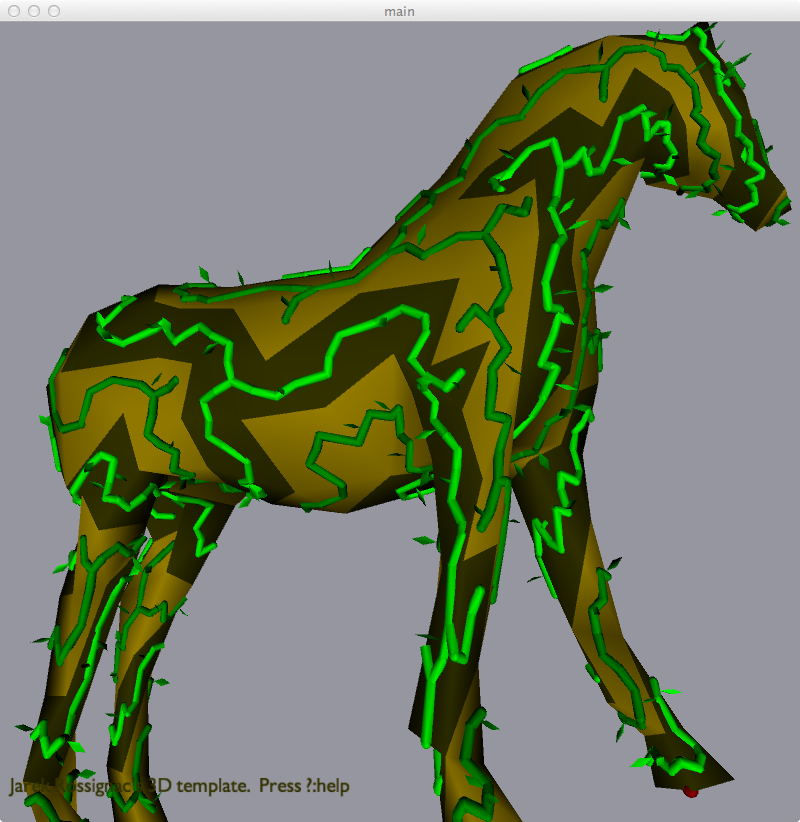
\includegraphics[width=3in]{data/vine}
\caption{Example of Vine around Horse}
\label{fig_angle}
\end{figure}

\section{Showing the vine}

The vine segments between triangle centers are drawn using  \verb+TRIANGLE_STRIP+.  Each vine segment is represented by some number of radial triangle strips.  In our examples, we used 12 radial segments in order to form the vine, which resulting in a fairly smooth shape that is visually pleasing.  

At the intersection of each vine segment, a smooth interface must be formed so that the vine looks continuous.  For this purpose, a sphere was drawn at each intersection. 

The vine leaves are drawn using \verb+TRIANGLE_FAN+. 

\section{Future Work}


A better canvas would make drawing easier.
One possibility is a plane on which balls can be placed on, or a choice between several starting configurations.
In addition, a toolbar style mode selection (Add Ball mode, Delete Ball mode) would make the application more user-friendly.

\begin{IEEEbiography}[{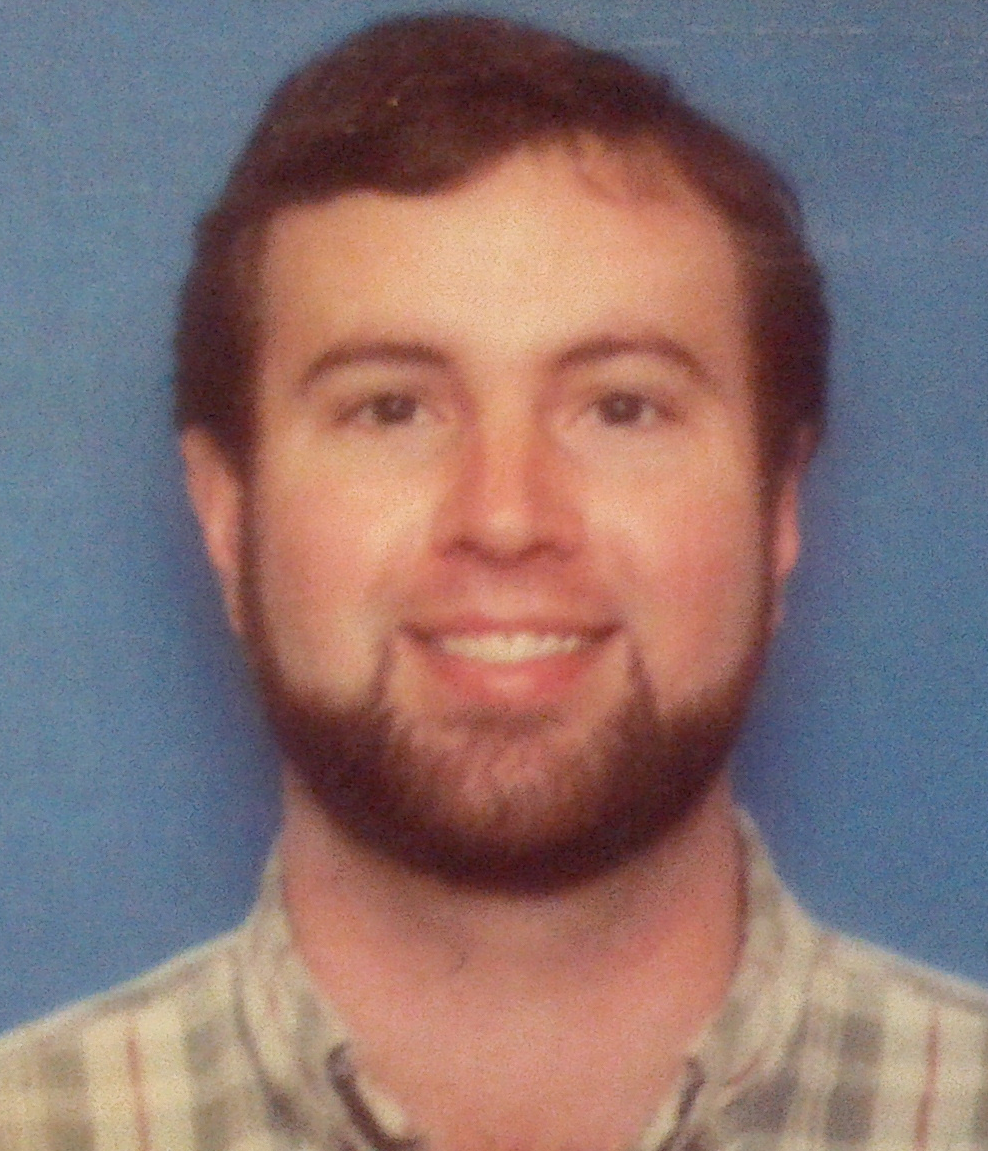
\includegraphics[width=1in,height=1.25in,clip,keepaspectratio]{data/dsmith.png}}]{Donnie Smith} donnie.smith@gatech.edu
\end{IEEEbiography}

\begin{IEEEbiography}[{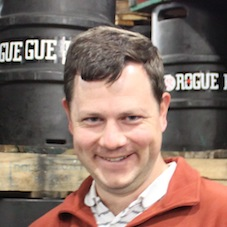
\includegraphics[width=1in,height=1.25in,clip,keepaspectratio]{data/kwharrigan.jpg}}]{Kyle Harrigan} kwharrigan@gatech.edu
\end{IEEEbiography}
\end{document}
